%%%%%%%%%%%%%%%%%%%%%%%%%%%%%%%%%%%%%%%%%
% NIWeek 2014 Poster by T. Reveyrand
% www.microwave.fr
% http://www.microwave.fr/LaTeX.html
% ---------------------------------------
% 
% Original template created by:
% Brian Amberg (baposter@brian-amberg.de)
%
% This template has been downloaded from:
% http://www.LaTeXTemplates.com
%
% License:
% CC BY-NC-SA 3.0 (http://creativecommons.org/licenses/by-nc-sa/3.0/)
%
%%%%%%%%%%%%%%%%%%%%%%%%%%%%%%%%%%%%%%%%%

%----------------------------------------------------------------------------------------
%   PACKAGES AND OTHER DOCUMENT CONFIGURATIONS
%----------------------------------------------------------------------------------------

\documentclass[a0paper,portrait]{baposter}

\usepackage[font=small,labelfont=bf]{caption} % Required for specifying captions to tables and figures
\usepackage{booktabs} % Horizontal rules in tables
\usepackage{relsize} % Used for making text smaller in some places

\usepackage{amsmath,amsfonts,amssymb,amsthm} % Math packages
\usepackage{eqparbox}

\usepackage{textcomp}

\usepackage{caption}
\usepackage{subcaption}
\usepackage{graphicx}
\usepackage{listings}
%\usepackage{verbatimbox}
%\usepackage{hyperref}

\usepackage{pgf}
\usepackage{tikz}
\usepackage[utf8]{inputenc}
\usetikzlibrary{arrows,automata}
\usetikzlibrary{positioning}


\graphicspath{{figures/}} % Directory in which figures are stored

 \definecolor{bordercol}{RGB}{40,40,40} % Border color of content boxes
 \definecolor{headercol1}{RGB}{186,215,230} % Background color for the header in the content boxes (left side)
 \definecolor{headercol2}{RGB}{120,120,120} % Background color for the header in the content boxes (right side)
 \definecolor{headerfontcol}{RGB}{0,0,0} % Text color for the header text in the content boxes
 \definecolor{boxcolor}{RGB}{210,235,250} % Background color for the content in the content boxes


\tikzset{
    state/.style={
           rectangle,
           rounded corners,
           draw=black, very thick,
           minimum height=2em,
           inner sep=2pt,
           text centered,
           },
}

\begin{document}

\setlength{\fboxsep}{0pt}

\background{ % Set the background to an image (background.pdf)
\begin{tikzpicture}[remember picture,overlay]
\draw (current page.north west)+(-2em,2em) node[anchor=north west]
{
\includegraphics[height=1.1\textheight]{background}};
\end{tikzpicture}
}

\begin{poster}{
grid=false,
columns=4,
borderColor=bordercol, % Border color of content boxes
headerColorOne=headercol1, % Background color for the header in the content boxes (left side)
headerColorTwo=headercol2, % Background color for the header in the content boxes (right side)
headerFontColor=headerfontcol, % Text color for the header text in the content boxes
boxColorOne=boxcolor, % Background color for the content in the content boxes
headershape=roundedright, % Specify the rounded corner in the content box headers
headerfont=\Large\sf\bf, % Font modifiers for the text in the content box headers
textborder=rectangle,
background=none,
headerborder=open, % Change to closed for a line under the content box headers
boxshade=plain
}
{
\includegraphics[width=3cm]{BiAtA2018.png}}
%
%----------------------------------------------------------------------------------------
%   TITLE AND AUTHOR NAME
%----------------------------------------------------------------------------------------
%
{ \bf  \huge {16s rRNA Detection by Using Context-Free Grammars and Neural Networks} }
%\\  \Large \it Context-free grammars and neural networks for secondary structure} % Poster title
{\vspace{0.3em} \smaller \textbf{Semyon Grigorev$^1$}, Polina Lunina$^1$ \\  % Author names
\smaller \it $^1${Saint Petersburg State University, JetBrains, St. Petersburg, Russia } \\ % Author email addresses
\smaller  {\textbf{E-mail:} semen.grigorev@jetbrains.com}}
{
\includegraphics[width=3cm]{SPbGU_Logo.png}} % University/lab logo


%----------------------------------------------------------------------------------------
%   INTRODUCTION
%----------------------------------------------------------------------------------------
\headerbox {Motivation}{name=introduction,column=0,row=0, span=2}{

Algorithms that can efficiently and accurately identify and classify bacterial taxonomic hierarchy have become a focus in computational genetics.
The idea that secondary structure of genomic sequences is sufficient for solving the detection and classification problems lies at the heart of many tools.%~\cite{GrammarsRNA, PCFG, LWPCFG}. 
The secondary structure can be specified in terms of formal grammars. 
The sequences obtained from the real bacteria usually contain a huge number of mutations and ``noise'' which renders precise methods impractical. 
Probabilistic grammars and covariance models (CMs) are a way to take the noise into account~\cite{EddyDurbin}.
For example, CMs are successfully used in the Infernal tool. %~\cite{Infernal}.
Neural networks is another way to deal with ``noisy'' data. 
The works~\cite{Humidor, ANN} utilize neural networks for 16s rRNA processing and demonstrate promising results.
In our work we want to combine ordinary context-free grammars nad neural networks and utilize this composition for 16s rRNA detecting and classification.
%\vspace{0.17cm}
}

\headerbox {Results}{name=results,column=2,row=0, span=2}{
\begin{itemize} 
\item We combine neural networks and ordinary context-free grammars to classify genomic sequences by using its secondary structure information. We extract features by using the ordinary (not probabilistic) context-free grammar and use the dense neural network for features processing.
\vspace{-0.2cm}
\item We evaluate the proposed approach for 16s rRNA detection. Current accuracy is 90\% for validation set (up to 81000 sequences from NCBI and Green Genes databases), thus we conclude that our approach is applicable. 
\vspace{-0.2cm}
\item Our solution provides an ability to use GPGPU and multi-core systems for sequences processing which can be useful for large biological data analysis.
\end{itemize}
\vspace{0.32cm}
}
    
\headerbox{Solution Overview}{name=CFParsing,span=4,column=0,row=1,below=introduction}{

\begin{tikzpicture}[->,>=stealth']


\node[state,
      align=left,
      text width = 7cm] (grm) 
 {
  \textbf{Grammar}\\
 \vspace{0.2cm}  
{\ttfamily
s1: stem<s0> any
\\
a\_0\_7 : any*[2..10]
\\
s0: a\_0\_7 | a\_0\_7 stem<s0> s0
\\
any: A | U | C | G
\\
stem1<s>: A s U | G s C | U s A | C s G 
\\    
stem2<s>: stem1< stem1<s> >
\\
stem<s>:  \\
\qquad      A stem<s> U \\
\qquad    | U stem<s> A \\
\qquad    | C stem<s> G \\
\qquad    | G stem<s> C \\
\qquad    | stem1< stem2<s> >  \\
 } 
 \vspace{0.2cm}
Fixed context-free grammar describes features of secondary structure and can be tuned in order to increase result quality.
 
 };


\node[state, 
      below of=grm,
      node distance=5.3cm,
      align = left,
      text width = 7cm] (sqs) 
 {
 \textbf{Sequences}\\
  \vspace{0.2cm}
Genoms parts of fixed length. Current length is 512. Length is variable parameter and can be changed in order to increase quality of solution.
Each sequence is treated as a text in $\{A, U, G, C\}$ alphabet.
 };


\node[state,
      right of=grm, 
      node distance=7.5cm,
      align = left,
      text width = 6cm](parser)
{
\textbf{Parser}\\
 \vspace{0.2cm}
Parser is features extractor: it extracts features of given squence secondary structure.
Parsing algorithm is based on the algorithm~\cite{gsv}, so the grammar can be extended with conjunctive rules~\cite{Okhotin} for pseudoknots description.%~\cite{zier2013rna}.
Parser performance is a bottleneck of our solution.
Current implementation utilizes GPGPU and should be optimized in future.
};

\node[state, 
      right of=parser,
      node distance=8cm,
      align = left,
      text width = 8.1cm] (mtrx) 
{
  \textbf{Matrices}\\
   \vspace{0.2cm}
{\centering
  \fbox{
\includegraphics[width=2.5cm]{figures/mt1.png}}
  \
  \fbox{
\includegraphics[width=2.5cm]{figures/mt2.png}}
  \
  \fbox{
\includegraphics[width=2.5cm]{figures/mt3.png}}
  }
\\
Parsing result is boolean (0-1) matrix which represents secondary structure features for sequence $\omega$: cell $[i,j]$ contains 1 iff $\omega.[j,i]$ is derivable from {\ttfamily s1} and $0$ in other case.
These matrices can be handled as images or binary vectors by using respective types of neural networks (convolutional or binary) and one of topics for future research is to select better approach. 
Currently we compress each matrix to integer vector and use dense newral network.
};

\node[state,
      below of=sqs, 
      node distance=3.5cm,
      align = left,
      text width = 7cm](result)
{
\textbf{Result of classification}\\
 \vspace{0.2cm}
Currently we implement only simple binary classifier that separates 16s and non-16s sequences.
One of interesting question is may this classifier be used for chimeric sequences filtering.
We hope that it is possible because ``global'' secondary structure of chimeric sequences should be broken.
};


\node[state,
      right of=result, 
      node distance=9cm,
      align = left,
      text width = 9.7cm](DNN)
{
\textbf{Neural Network}\\
 \vspace{0.2cm}
\begin{minipage}[t]{5.5cm}
We use dense neural network with 14 dense layers.
Almost all of them are wrapped with dropout (up to 75\%) and batch normalization layers for learning stabilization.
Our network is trained on up to 310000 sequences of length 512: positive (16s rRNA) from NCBI database, negative (non-16s) from Green Genes database.
Current accuracy for validation set (up to 81000 sequences) is 90\%. 
\end{minipage}
\begin{minipage}[t]{4cm}
Typical building block:
\\
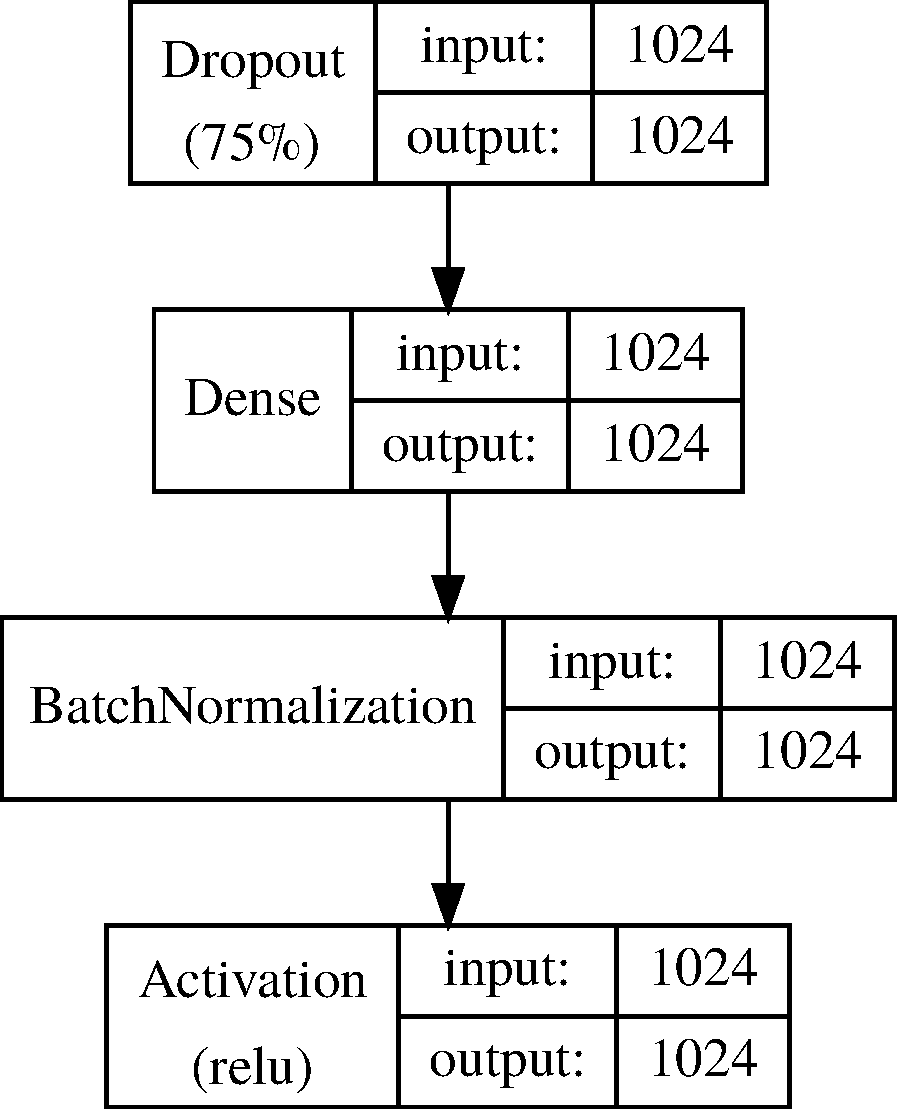
\includegraphics[width=4cm]{figures/bb.pdf}
\end{minipage}


};


\node[state,
      right of=DNN, 
      node distance=8cm,
      align = left,
      text width = 5cm](vector)
{
\textbf{Vectors}\\
\vspace{0.2cm}
We use line-by-line compressed matrix representation: sequence of 32 cells (bits) is compressed to unsigned integer. 
Top right triangle of matrix is always empty, so can be ignored. 
We hope that compression to 16 bit integer or byte may decrease complexity of neural network and improve result quality, but it requires significantly more memory on GPGPU which can be serious technical problem.

};


\path (grm) edge  (parser)
 (sqs) edge [bend right] (parser)
% (sqs) edge (parser)
 (parser) edge (mtrx)
 (mtrx) edge (vector)
 (vector) edge (DNN)
 (DNN) edge (result)
 ;

\end{tikzpicture}


}

\headerbox {Future Research}
{name=app1,column=0,span=2, below=CFParsing}
{ 
The presented is a work in progress. 
The ongoing experiment is finding all instances of 16s rRNA in full genomes.
Also we plan to use the proposed approach for the filtration of chimeric sequences and the classification.
Composition of our approach with other methods and tools as well as grammar tuning and detailed performance evaluation may improve the applicability for the real data processing.
}

%----------------------------------------------------------------------------------------
%   REFERENCES
%----------------------------------------------------------------------------------------

\headerbox {References}
{name=app2,column=2,span=2, below=CFParsing}
{
\smaller % Reduce the font size in this block
\renewcommand{\section}[2]{\vskip 0.05em} % Get rid of the default "References" section title
%\nocite{*} % Insert publications even if they are not cited in the poster

\bibliographystyle{unsrt}
%\bibliographystyle{IEEEtran}
\bibliography{biblio} % Use biblio.bib as the bibliography file
}



\headerbox {Acknowledgments}{name=ack,column=0,span=1,below=app1}{
The research was supported by the Russian Science Foundation grant 18-11-00100 and a grant from JetBrains Research.
\vspace{0.24cm}
}
    
\headerbox {Information}{name=info,column=1,span=1,below=app1}{
All materials available on GitHub: \small{https://github.com/YaccConstructor}
\vspace{0.68cm}
}


\end{poster}

\end{document}
